\documentclass[../main.tex]{subfiles}

\begin{document}
The alignment algorithm has been thoroughly tested using both synthetic and experimental datasets. The benefit of using synthetic data to assess alignment algorithms is that the ground truth values of the alignment parameters are known. As a consequence, any discrepancy in the output of the alignment algorithm can be attributed as an error of the alignment algorithm. In spite of this, the synthetic data is usually generated using a naive model of the microscope. Therefore, results obtained with synthetic data may not reflect the real performance of the algorithm. To address this issue, the algorithm has also been tested with experimental data.

The datasets used for our tests were selected to reflect proteins with a diverse set of characteristics, such as symmetry, size, presence of membrane, flexible parts\dots In total, 4 proteins were selected. Each of these proteins will be tested with both simulated and experimental data.

\subsection{Synthetic Data}
The synthetic datasets used to test the algorithm were generated from \gls{pdb} files using the Scipion framework\cite{delarosa2016}. \Gls{pdb} files contain the atomic model description of the protein. Therefore, the first step is to render a volume from this model. This can be easily achieved using the \texttt{xmipp3 - convert a PDB} protocol. This volume can now be used to generate projections as the microscope would do. 

The volume is then projected from all directions using \texttt{xmipp3 - create gallery} leading to a set of clean projections of the volume. However, these projections do not reflect well experimental images due to the absence of noise. Therefore, some amount of \gls{agwn} is added to the images through the \texttt{xmipp3 - add noise particles} protocol to simulate ice particles in the sample. This noise has zero mean and its standard deviation will be selected in such a way that the \gls{snr} of the image is $-10 \si{\decibel}$. Lastly, a \gls{ctf} is applied to the images using \texttt{xmipp3 - simulate CTF} protocol. 

In total, $41219$ projections will be generated from equally spaced orientations. This ensures that the algorithm will be tested with all possible orientations of the protein. Additionally, the particles will be shifted in-plane by a normal distribution of $\sigma=6\si{px}$. Therefore, $95\si{\percent}$ of the images will contain a shift of less than $12 \si{px}$, which is a reasonable value. Similarly, the defocus parameter of the \gls{ctf} will be uniformly chosen for each particle in the range of $5000 \si{\angstrom}$ to $25000 \si{\angstrom}$.

\subsection{Experimental Data}
The experimental images used in these tests were obtained from \gls{empiar}. \Gls{empiar} is a public archive maintained by the \gls{embl}-\gls{ebi} which provides open access to raw \gls{cryoem} images\cite{iudin2022}. Among other things, this initiative enables testing \gls{cryoem} image processing algorithms with a wide variety of real data.

Some of the selected datasets provided extracted particles, which are the starting point of the alignment algorithm. However, some others only provided micrographs or movies. In those cases, the data needed to be processed before being suitable for our use case. This processing was done inside the Scipion framework. Depending on the dataset, movie alignment, \gls{ctf} estimation, particle picking and particle extraction steps needed to be carried out to obtain the desired particles.

To address the fact that the alignment information of the experimental images is not known, these particles were aligned using Relion\cite{scheres2021} and Cryosparc\cite{cryosparc}. Then, their outputs were consensuated so that only particles that coincided below a threshold are considred. This gives some amount of confidence to the estimated alignment of the particles, as two independent algorithms coincided in the result. Nevertheless, these parameters do not need to be the ground truth.

\subsection{Test proteins}
\subsubsection{EMPIAR-10028}
This acquisition is related to the Plasmodium falciparum, which is present in the human malaria parasite\cite{wong2014}. This dataset is widely used when testing \gls{cryoem} algorithms.

As stated earlier, alignment algorithms use particles and a volume as the starting point. Although individual particles are provided in the dataset, these particles were obtained several years ago. Therefore, we preferred to obtain the particles from scratch using modern methods so that we can take advantage of state of the art techniques.

\subsubsection{EMPIAR-10061}
The \gls{empiar}-10061 dataset is an aquisition of the $\beta$-galactosidase protein. Similarly to the prior dataset, this dataset is also widely used when assesing \gls{cryoem} algorithms. 

The particularity of this dataset is that it has $D2$ symmetry. This is important when aligning, because it reduces the number of possible projection angles. Moreover, each experimental image can be used to fill multiple planes in Fourier space when reconstructing, which usually increases \gls{snr}. 

\subsubsection{EMPIAR-10256}
This dataset is  a TRPV5 with calmodulin bound \gls{cryoem} acquisition\cite{dang2019}. 

\subsubsection{EMPIAR-10391}
This dataset refers to a Arabinofuranosyltransferase AftD from Mycobacteria \gls{cryoem} acquisition. This protein is responsible of causing the tuberculosis decease, which kills over 1 million people every year\cite{tan2020}.

The dataset is distributed either in the form of movies or a particle stack. As mentioned earlier, the later one suits better our needs, as the input for the alignment algorithm is a particle stack.

The aim of the experiment was to test a drug binding to the protein. Hence, the dataset is heterogeneous, this is, some particles may originate from the clean protein and some others may originate from the protein with the drug bound. As the dataset reflects two structures, two atomic models were fitted into it. Therefore, this dataset can be used to test if the algorithm is able to distinguish discrete 3D classes. 

Another peculiarity of this dataset is that the protein is that it is embedded in a membrane. As the membrane structure is highly flexible and does not follow a specific pattern, these type of proteins tend to be difficult do align.

Figure \ref{fig:5:empiar10391} shows a small subset of the visual aspect of the experimental and simulated images belonging to this dataset.

\begin{figure}[htbp]
    \centering
    \begin{subfigure}[b]{0.45\textwidth}
         \centering
         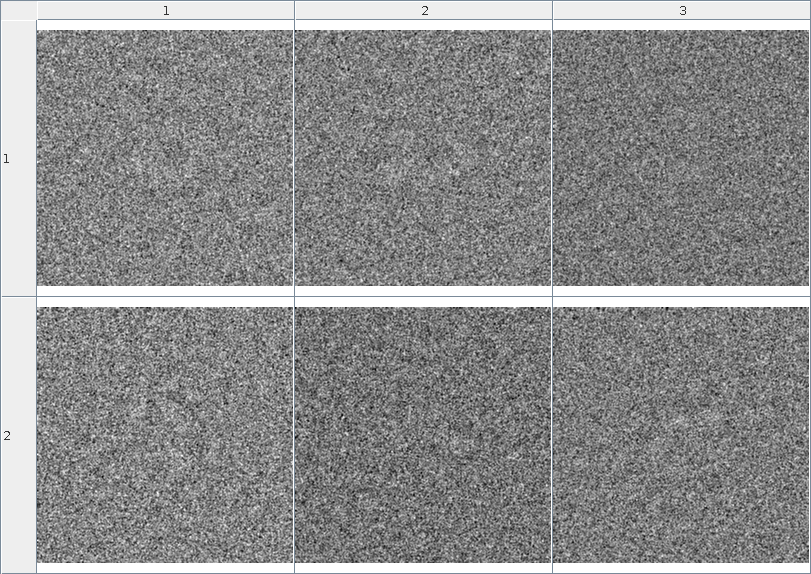
\includegraphics[width=\linewidth]{results/datasets/empiar10391/phatoms}
         \caption{Simulated images}
    \end{subfigure}
    \hfill
    \begin{subfigure}[b]{0.45\textwidth}
         \centering
         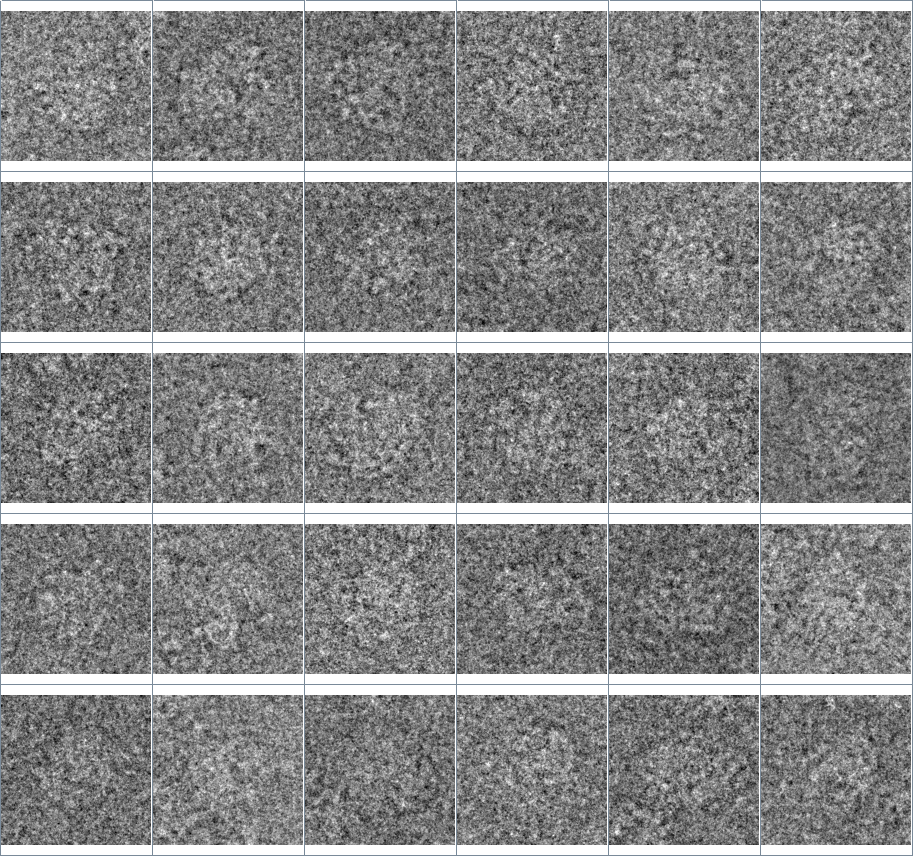
\includegraphics[width=\linewidth]{results/datasets/empiar10391/experimental}
         \caption{Experimental images}
    \end{subfigure}\\
    \caption{Visual aspect of experimental and simulated images of EMPIAR 10391}
    \label{fig:5:empiar10391}
\end{figure}


\begin{table}[hbtp]
    \centering
    \begin{tabular}{|l|c|}
        \hline
        Pixel size & $1.0605 \si{\angstrom/px}$ \\\hline
        Particle dimensions & $256\times256 \si{px^2}$ \\\hline
        Particle count & $106045$ \\\hline
    \end{tabular}
    \caption{Characteristics of EMPIAR-10391 dataset}
    \label{tab:5:empiar10391}
\end{table}

\end{document}